
\chapter{Related Work}
\label{chap:literature}
This chapter delves into an in-depth exploration of existing research and developments in the field of battery-less IoT devices, intermittent connectivity solutions, and the pivotal role of the FreeBie architecture. By examining advancements, challenges, and critical gaps in the literature, this section lays the foundation for understanding the significance of the proposed CardioSync framework.

% The subsequent sections discuss key areas of interest, shedding light on the evolving landscape of battery-less IoT and intermittent communication in the context of modern technological demands. Additionally, the advancements and interesting researches in the field of Body Sensor Networks is also explored in the context of Energy demand and need for energy efficient computing. This aids to justify the application of our thesis, as it is aimed for Body sensor network owing to the use of Heart rate sensor.

\section{Battery-Free IoT for Wireless Sensor Networks}
The field of battery-less IoT has garnered significant attention, driven by the promise of sustainable, autonomous operation. This approach offers extended device lifetimes and reduced environmental impact. Researchers and innovators have actively explored diverse energy harvesting techniques to power these devices, enabling applications across various domains such as agriculture, logistics, and environmental monitoring. Early works like the development of wireless sensor networks using simple solar energy harvesters and cost-effective energy storage units \cite{4394148} laid the groundwork for the subsequent advancements.
\vspace{1\baselineskip}

\noindent A notable milestone was achieved in 2017, the integration of solar energy harvesting chips and super capacitors in a battery-less sensor tag \cite{7990978} showcased the successful integration of multiple sensors, including temperature, humidity, and gas sensors, with efficient data transmission through BLE communication. This advancement proved particularly promising for industrial applications, hinting at the viability of battery-less IoT in various sectors. In 2020 with the introduction of a system utilising ambient RF energy to power battery-less tags \cite{10.1145/3386901.3396604} highlighted the potential of harnessing ubiquitous energy sources for practical applications. Intriguingly, the employment of a piezoelectric converter as an energy harvester to power a Bluetooth board through low-voltage vibration electromagnetic conversion was explored \cite{9221051}. This exploration validates the spectrum of solutions available to enhance the battery-less capability of IoT devices while still facilitating the formation of sensor networks. 
\vspace{1\baselineskip}

\noindent A distinct stride was taken towards achieving batteryless communication through the successful design and testing of a wireless LoRaWAN end sensor node \cite{9299539}. This innovative approach demonstrates the feasibility of battery-less IoT even in long-range communication scenarios, further expanding the scope of its potential applications.
\vspace{1\baselineskip}

\noindent These strides exemplify only a subset of the numerous breakthroughs within the domain of battery-free IoT wireless communication. The works \cite{9718062}, \cite{10101211}, \cite{10.1145/3276774.3282823} offer additional evidence of the expanding landscape of battery-free IoT. Collectively, these advancements illuminate the dynamic landscape of battery-free IoT, highlighting its capacity to revolutionise myriad domains, from conventional industries to cutting-edge technologies.

\subsection{The FreeBie}
\label{sec:freebie_architecture}

\begin{figure}[t]
    \centering
    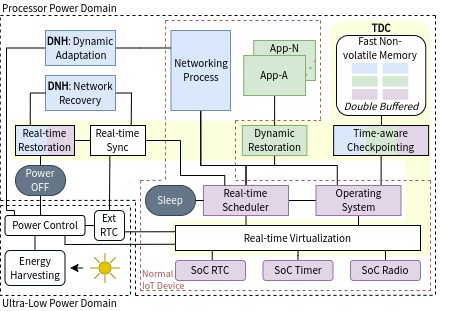
\includegraphics[width=0.6\linewidth]{chapters/Literature/diagram.jpg}
    \caption{FreeBie Architecture \cite{de2022Intermittently}.}
    \label{fig:freebie_paper_arch}
\end{figure}
\begin{figure}[t]
    \centering
    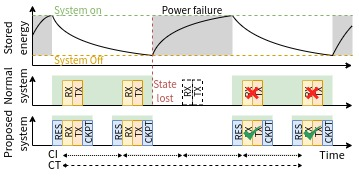
\includegraphics[width=0.6\linewidth]{chapters/Literature/intro.jpg}
    \caption{Conceptual illustration of intermittently-powered communication device operation. In normal system, a power outage results in a disruption of the connection and necessitates additional handshakes to reestablish and configure the connection. The FreeBie system has a checkpointing and restoration mechanism that utilises nonvolatile memory for the purpose of storing network state and sustain connections, even in the event of a power outage. CT: connection timeout; CI: connection interval; RES: state restore; CKPT: state checkpoint; RX/TX: reception/transmission \cite{de2022Intermittently}.}
    \label{fig:freebie_paper_conn}
\end{figure}

In the realm of intermittent connectivity solutions, the FreeBie architecture emerges as a pivotal contender, offering a distinctive approach to achieving Bluetooth Low Energy (BLE) communication on intermittently-powered wireless devices \cite{de2022Intermittently}. This architecture, shown in Figure \ref{fig:freebie_paper_arch}, introduces an adaptive framework that tailors connection parameters according to the available harvested energy, facilitating efficient communication in resource-constrained environments. One of its significant features is to maintain BLE connections despite intermittent power, as illustrated in Figure \ref{fig:freebie_paper_conn}. Its unique ability to enable bi-directional communication and dynamically manage network connections fills a critical gap in the domain of intermittently-powered devices. Also it supports preemptive scheduling, allowing network processes to take precedence over application or operating system processes.
\vspace{1\baselineskip}

\noindent These components within FreeBie architecture serve a critical role on achieving the battery less operation:
\begin{itemize}
    \item \textbf{FRAM (Ferroelectric RAM):} FRAM is a non-volatile memory technology that offers high read/write speeds and low power consumption. It stores data and program code, ensuring persistence during power cycles. FRAM preserves memory sections during each checkpoint and stores context across separate allocated regions for OS processes, Network processes, and Application processes.
    
    \item \textbf{External RTC (Real-Time Clock):} The external RTC provides accurate timekeeping even during device power-off periods. This time reference is vital for synchronisation and event scheduling. The external RTC remains always powered through onboard capacitors and can control processor power domains using the Power switch and Power control module.
    
    \item \textbf{Time-Deterministic Checkpointing and Restore:} This component maintains data integrity by regularly capturing the device's state. In cases of power disruptions, the system can restore to a known state, preventing data loss and ensuring system consistency. It leverages External RTC and FRAM for uninterrupted atomic operations.
    
    \begin{itemize}
        \item \textit{Real-time RTC sync:} This subcomponent synchronises the Ext. RTC with the onboard RTC during each real-time operation resumption from power-off state. It uses FRAM to store the synchronising time \(T_{Sync}\) in the OS context.
        \item \textit{Real-time/Dynamic Restoration:} Upon resuming from power-off state, this component restores processes from FRAM for OS processes, network processes, and real-time application processes, as scheduled by the scheduler.
        \item \textit{Dynamic Handling of Network Connection:} Responsible for network recovery and dynamic network adaptation, this subcomponent ensures network recovery in unexpected power-offs and adapts to energy conditions while maintaining connection.
    \end{itemize}
    
    \item \textbf{Power Control:} Governing power state transitions, power control mechanisms by managing power-on timings, task execution, and low-power modes.
    
    \item \textbf{Super Capacitors and Energy Harvesters:} Integral to FreeBie's energy autonomy, super capacitors and energy harvesters contribute to storing and harnessing energy from ambient sources.
\end{itemize}

\noindent However, since the architecture relies on external components such as FRAM and an external RTC, it impacts factors like system cost, size, and energy consumption. To address this, the authors suggest future exploration into developing a FreeBie version that integrates next-generation System on Chip (SoC) technology and leverage more energy-efficient harvesters.
\vspace{1\baselineskip}

\noindent Furthermore, the FreeBie architecture is designed to support intermittently-powered end devices, but a notable research gap lies in the absence of support for intermittently-powered hosts on both sides of BLE communication. While the architecture excels in enabling communication between intermittently-powered device and continuously powered hosts, there's potential for innovation in extending its capabilities to encompass two intermittently-powered end nodes. This extension could unlock novel use cases in wireless sensor networks, broadening the applicability of the FreeBie architecture.

\section{Body Sensor Network}
The evolution of Body Sensor Networks (BSNs) has marked a significant milestone in healthcare and wellness monitoring. These networks, composed of wearable sensors, offer real-time data collection, analysis, and transmission, empowering individuals and healthcare professionals with valuable insights into physiological and medical conditions. BSNs demonstrated remarkable potential in applications ranging from remote patient monitoring to sports performance analysis and beyond.
\vspace{1\baselineskip}

\noindent Early research in BSNs primarily focused on sensor integration and data aggregation techniques \cite{5678072}. These studies paved the way for more advanced BSNs capable of real-time health monitoring. The advent of wearable devices with integrated physiological sensors has led to the development of innovative solutions for continuous monitoring of vital signs such as heart rate, temperature, and electrocardiogram (ECG) signals \cite{BSNreview}, \cite{6555588}. These advancements enable early detection of anomalies and timely intervention in critical situations.
\vspace{1\baselineskip}

\noindent The energy requirements of BSNs vary based on the complexity of sensors and the data transmission frequency. Wearable sensors that capture high-resolution data, such as ECG signals, demand a continuous power source for accurate monitoring. However, battery limitations hinder the potential for uninterrupted data collection. This challenge becomes even more pronounced when considering the size and weight restrictions of wearable devices \cite{WANG2020112410}, \cite{4755157}, \cite{6755575}.
\vspace{1\baselineskip}

\noindent The integration of battery-free IoT devices within BSNs offers a promising solution to the energy challenge \cite{5370806}. This innovation not only extends the operational lifetime of BSNs but also opens the door to continuous and sustainable monitoring. Also it could be affordable (less than US\$2 each when manufactured in volume), disposable, small, and easy to use \cite{5370806}. Although there are already some Battery free Wireless BSN solutions but they do use near-field-enabled clothing capable of establishing wireless power and data connectivity between multiple distant points around the body to create a network of battery-free sensors interconnected by proximity to functional textile patterns.\cite{Lin_Kim_Achavananthadith_Kurt_Tan_Yao_Tee_Lee_Ho_2020}
\vspace{1\baselineskip}

\noindent In summary, the evolution of BSNs has been characterised by breakthroughs in sensor integration and wireless communication. However, the challenge of battery dependence has persisted. The emergence of battery-free IoT devices powered by energy harvesting techniques presents a transformative solution. As ongoing research continues to address energy challenges and optimise device performance, the future of BSNs holds the promise of continuous and sustainable healthcare monitoring.